\documentclass{beamer}
\usepackage[utf8]{inputenc}
\usepackage[spanish]{babel}
\usepackage{subfigure, wrapfig}
\usepackage{multirow}
\usepackage{hyperref} %referencia


\date{} %not show date

%beamer's options
\usetheme{Montpellier}
\author{Gustavo Rivas Gervilla}
\title{Lógica difusa en la descripción lingüística de datos}
\subtitle{LDD, series temporales y búsqueda de expresiones de referencia}
\institute{
	Escuela Técnica Superior de Ingeniería Informática y Telecomunicaciones	
}

\setbeamertemplate{section in toc shaded}[default][50]
%beamer's colors
\setbeamercolor{section in toc}{fg=orange}
\setbeamercolor{section in toc shaded}{fg=orange}
\setbeamercolor{structure}{fg=brown}
\setbeamercolor{title}{fg=brown}
\setbeamercolor{titlelike}{fg=brown}

\newtheorem{definicion}{Definición}
\newtheorem{proposicion}{Proposición}

\begin{document}
	\begin{frame}[plain]
		\titlepage
	\end{frame}
	
	\begin{frame}[plain]
		\frametitle{Contenido}
		\tableofcontents
	\end{frame}
	
	\AtBeginSection[]{
		\begin{frame}[plain]
			\frametitle{Contenido}
			\tableofcontents[currentsection]
		\end{frame}
	}
	
	\section{Introducción}
	
	\begin{frame}
		Gran cantidad de información $\longrightarrow$ usuarios no expertos.
		
		\begin{itemize}
			\item \textbf{NLG:} generación de textos que proporcionan información indistinguibles de los producidos por un humano.
			\item \textbf{LDD:} proporciona descripciones de conjuntos de datos empleando concepctos lingüísticos definidos mediante conjuntos difusos.
		\end{itemize}		
	\end{frame}
	
	\begin{frame}
		\begin{itemize}
			\item \textbf{Determinación del contenido:} decidir qué información se ha de comunicar por medio del texto a crear.
			\item \textbf{Planificación del discurso:} dar un orden y una estructura al conjunto de mensajes a verbalizar.
			\item \textbf{Agrupación de oraciones:} agrupar varios mensajes en una sola oración. (opcional)
			\item \textbf{Lexicalización:} decidir qué palabras y expresiones han de usarse.
			\item \textbf{Generación de las expresiones de referencia (referring expression):} seleccionar las palabras o expresiones que identifican las entidades del dominio.
			\item \textbf{Realización lingüística:} aplicar reglas gramaticales para producir un texto que sea sintácticamente, morfológicamente y ortográficamente correcto a partir de los elementos anteriormente generados.
\end{itemize}
	\end{frame}
	
	\section{LDD}
	
	\begin{frame}
		Surge a partir de las ideas de Zadeh y Yager. Usar la lógica difusa para realizar computación con palabras (CW).\\
				
		CW $\longrightarrow$ resumen lingüístico de datos.
		
		\begin{itemize}
			\item Flujo de pacientes.
			\item Consumo doméstico de electricidad.
			\item Actividad humana basada en acelerómetros de móviles.
			\item Meteorología.
		\end{itemize}
		
		Es un campo relativamente moderno con lo que no hay una técnica general para cualquier tipo de problema.
	\end{frame}
	
	\begin{frame}
		Dataset $\longrightarrow$ Extraer información  $\longrightarrow$ Representarla mediante conceptos lingüísticos.
		
		\begin{itemize}
			\item Los \textbf{datos de entrada}.
			\item \textbf{Variables lingüísticas}.
			\item \textbf{Cuantificadores difusos}.
			\item \textbf{Criterio de evaluación}.
		\end{itemize}
		
		Generar todas las posibilidades $\Rightarrow$ heurísticas y meta-heurísticas.
	\end{frame}
	
	\begin{frame}
		\begin{itemize}
			\item Campo muy teórico.
			\item Se pretende diseñar un framework de propósico general.
			\item Modelo granular de un fenómeno (GLMP) de Trivino y Sugeno: nodos con distintos niveles de abstracción interconectados entre sí.
		\end{itemize}		
	\end{frame}
	
	\section{Series temporales}
	
	\begin{frame}
		\begin{itemize}
			\item Mucha información en forma de \textbf{series temporales}.
		
			\item El proceso descripción lingüística de una serie temporal tiene dos partes:
				\begin{itemize}
					\item Extracción del conocimiento.
					\item Proceso de expresión lingüística.
				\end{itemize}
				
			\item La teoría de conjuntos difusos es especialmente útil para representar patrones imprecisos y modelar y procesar varios tipos de imprecisión e información incompleta.
		\end{itemize}
	\end{frame}
	
	\subsection{Generación de descripciones lingüísticas de series temporales}
	
	\begin{frame}
		\begin{itemize}
			\item Influenciado por el experto, el diseñador y el destinatario.
			\item Se genera un conjunto de mensajes que en conjunto describirán la serie temporal $\Rightarrow$ formalismo de representación del conocimiento.
			\item Espacio de búsqueda grande $\Rightarrow$ \textit{framework} de calidad.
		\end{itemize}
	\end{frame}
	
	\subsection{Formalismo de representación del conocimiento}
	
	\begin{frame}
		\begin{itemize}
			\item Nos centramos en el paradigma de la CW.
			\item \textbf{protoforma}: prototipo abstracto.
			\item Destacamos dos protoformas muy empleadas en este ámbito:
				\begin{itemize}
					\item $X \; es \; A$
					\item $Q \; D \; son \; A$
				\end{itemize}
		\end{itemize}
	\end{frame}
	
	\begin{frame}
		\begin{itemize}
		\item El formalismo da la semántica del mensaje a partir de la semántica de las protoformas que lo forman.
		\item La mayoría de las veces entre las 12 y las 15 horas el precio es constante. Su semántica viene dada por la de:
			\begin{itemize}
				\item La protoforma $Q \; D \; son \; A$.
				\item El componente \textit{entre las 12 y las 15 horas}.
				\item El componente \textit{constante}.
				\item El componente \textit{la mayoría de las veces}.
			\end{itemize}
		\end{itemize}
	\end{frame}
	
	\subsection{Técnica de extracción}
	
	\begin{frame}
		\begin{itemize}
			\item Serie temporal $\longrightarrow$ Conjunto de mensajes.
			\item En este proceso hay dos operaciones principales:
				\begin{itemize}
					\item Generación de nuevas series temporales.
					\item Búsqueda en el espacio semántico.
				\end{itemize}
			\item En principio el espacio semántico tiene una dimensión exponencial a la dimensión al espacio de instancias $\Rightarrow$ técnicas heurísticas $\Rightarrow$ técnicas jerárquicas.
		\end{itemize}
	\end{frame}
	
	\subsection{Proceso de expresión lingüística}
	
	\begin{frame}
		\begin{itemize}
			\item Conjunto de mensajes $\longrightarrow$ Texto para el usuario.
			\item No se pueden tener en cuenta las restricciones de cada tipo de usuario.
			\item Hay dos técnicas principales:
				\begin{itemize}
					\item \textbf{Basadas en plantillas}. La mayoría de técnicas usan unas pocas protoformas predefinidas.
					\item \textbf{\textit{Reales}}.
				\end{itemize}
		\end{itemize}
	\end{frame}
	
	\subsection{Framework de calidad}
	
	\begin{frame}
		\begin{itemize}
			\item Definir un framework de calidad es muy complejo, sobre todo para sistemas de propósito general. Esto es así porque:
			\begin{itemize}
				\item Una parte de la medida de calidad es claramente subjetiva y depende del contexto.
				\item La calidad de una descripción lingüística tiene muchos aspectos distintos, llamados \textbf{dimensiones de calidad}.
				\item Puede ocurrir que muchas de estas dimensiones estén fuertemente relacionadas, mientras que otras sean contradictorias entre sí.
			\end{itemize}
		\end{itemize}		
	\end{frame}
	
	\subsection{Aplicaciones}
	
	\begin{frame}
		\begin{itemize}
			\item En el campo del cuidado cardíaco podemos mencionar por ejemplo el sistema BT-45 que genera resúmenes textuales a partir de datos de sensores de una unidad de cuidados intensivos de recien nacidos.
			\item En el campo de la meteorología tenemos el sistema SUMTIME-MOUSAM que genera pronósticos meteorológicos a partir de datos números de predicciones meteorológicas.
			\item También hay sistemas centrados en el mercado bursátil.
			\item Sistemas que generan descripciones lingüísticas de un fenómeno ecológico como es el consumo doméstico de energía.
\end{itemize}
	\end{frame}
	
	\section{App}
	
	\begin{frame}
		Señala el triángulo verde.
		
		\begin{figure}[H]
			\centering
			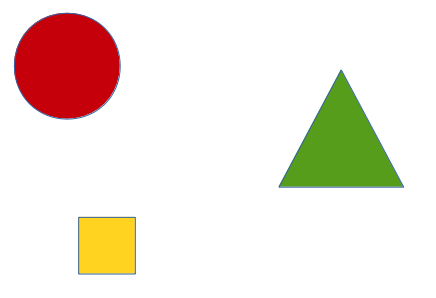
\includegraphics[width=40mm]{img/ejemplo1.png}			
		\end{figure}
	\end{frame}
	
	\subsection{Redes de información}
	
	\begin{frame}
		\begin{itemize}
			\item El proceso de expresiones de referencia puede aplicarse a muchos dominios distintos.
			\item Las rexp. se forman teniendo en cuenta la información que tenemos de los objetos de la escena.
			\item Es necesario un mecanismo de representación del conocimiento.
		\end{itemize}
	\end{frame}
	
	\begin{frame}
		\begin{figure}[H]
			\centering
			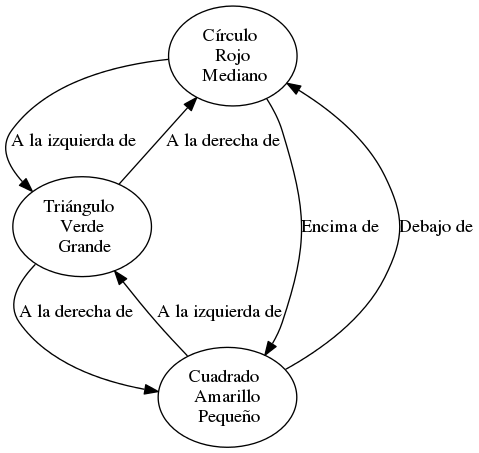
\includegraphics[scale=0.4]{img/RIejemplo1.png}
		\end{figure}
	\end{frame}
	
	\begin{frame}
		\begin{itemize}
			\item Emplear la estructura de grafo nos permite aprovechar su potencial.
			\item Trabajamos con propiedades difusas $\Rightarrow$ Grados de cumplimiento $\Rightarrow$ Escala de intensidad.
			\item Para las propiedades difusas usuales tenemos el [0,1].
		\end{itemize}
	\end{frame}
	
	\subsection{Problema}
	
	\begin{frame}
		\begin{itemize}
			\item Conjunto de objetos $\lbrace x_1, ..., x_n\rbrace$.
			\item Encontrar una combinación de propieadades $re = \lbrace p_1, ... p_n \rbrace$ con éxito referencial.
			\item Propiedades difusas $\Rightarrow$ Buscar en cada $\alpha$-corte $\Rightarrow$ Unificar los resultados.
		\end{itemize}
	\end{frame}
	
	\subsection{Medida de calidad}
	
	\begin{frame}
		\begin{itemize}
			\item La medida en la cual el conjunto de objetos a los que se les puede aplicar la expresión de referencia está compuesto únicamente por el objeto al que realmente se quiere identificar.
			\item Proponemos las siguientes propiedades para una medida de éxito referencial:
				\begin{enumerate}
					\item $rs(re, x) = 1 \; sii \; X_{re} = \lbrace x \rbrace$.
					\item Si $X_{re}(x) = 0$ entonces $rs(re, x) = 0$.
					\item Si $X_{re}(y) \leq X_{re'}(y), \forall y \in X\setminus\lbrace x\rbrace$ y $X_{re}(x) \geq X_{re'}(x)$ entonces $rs(re, x) \geq rs(re', x)$.
				\end{enumerate}
		\end{itemize}
	\end{frame}
	
	\begin{frame}
		\begin{definicion}
			Sea $re = \lbrace p_1,...p_n\rbrace$ una rexp. compuesta por propiedades difusas, $\alpha \in [0,1]$ y un objeto $x \in X$. Diremos que \textbf{$re$ tiene éxito referencial en el nivel $\alpha$ para el objeto $x$} sii:

			\begin{center}
				$\underset{p_i \in re}{\bigcap}[[p_i]]_\alpha = \lbrace x \rbrace$
			\end{center}
		\end{definicion}
	\end{frame}
	
	\begin{frame}
		\begin{definicion}
			El \textbf{conjunto de validez} de $re$ para el objeto $x$ es el conjunto de valores $\alpha$ en los que la rexp. tiene éxito referencial con respecto a $x$. Formalmente definimos este conjunto como sigue:
			\begin{center}
				$V_{re}^x = \left\lbrace \alpha \in [0,1] \mid \underset{p_i \in re}{\bigcap}[[p_i]]_\alpha = \lbrace x \rbrace \right\rbrace$
			\end{center}
		\end{definicion}

		Veamos un resultado relacionado con estos conjuntos de validez:

		\begin{proposicion}
			Si $V_{re}^x \neq \emptyset$ entonces es un intervalo.
		\end{proposicion}
	\end{frame}
	
	\begin{frame}
		Cuanto más grande sea $\alpha_1$, mayor será la veracidad de la rexp. para $x$. Y cuanto menor sea $\alpha_2$, menor será esta veracidad para el resto de objetos. En base a esto damos la siguiente definición de medida de éxito referencial, para una rexp. $re$ y un objeto $x$:

		\begin{definicion}
		\label{def: medida}
			$rs(re, x) = \left\lbrace 
			\begin{array}{ll}
      			\alpha_1(\alpha_1 - \alpha_2) \; \mathrm{si} \; V_{re}^x \neq \emptyset\\      
      			0 \; \mathrm{en \, otro \, caso}\\
			\end{array} \right.$
		\end{definicion}
	\end{frame}
	
	\subsection{Algoritmo}
	
	\begin{frame}
		\begin{figure}[H]
			\centering
			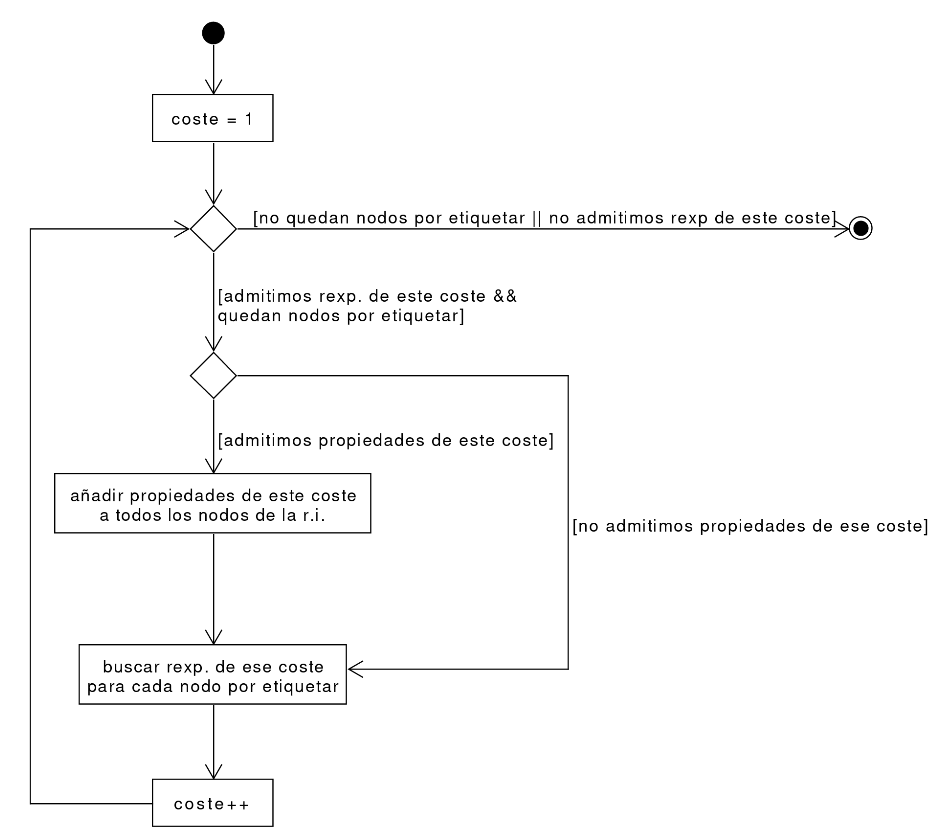
\includegraphics[scale=0.3]{img/diagramaFlujoAlgCrisp.png}
		\end{figure}
	\end{frame}
	
	\begin{frame}
		\begin{figure}[H]
			\centering
			
\includegraphics[width=0.55\textwidth]{img/ejemploAlgoritmoNoDifuso.png}
			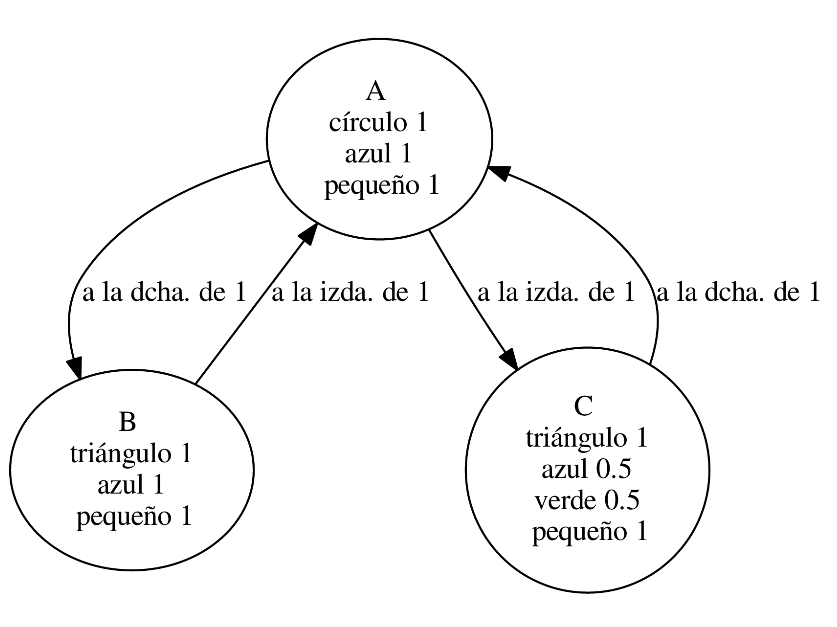
\includegraphics[width=0.6\textwidth]{img/riEjemploAlgoritmoNoDifuso.png}		
		\end{figure}		
	\end{frame}
	
	\begin{frame}
		\begin{figure}
			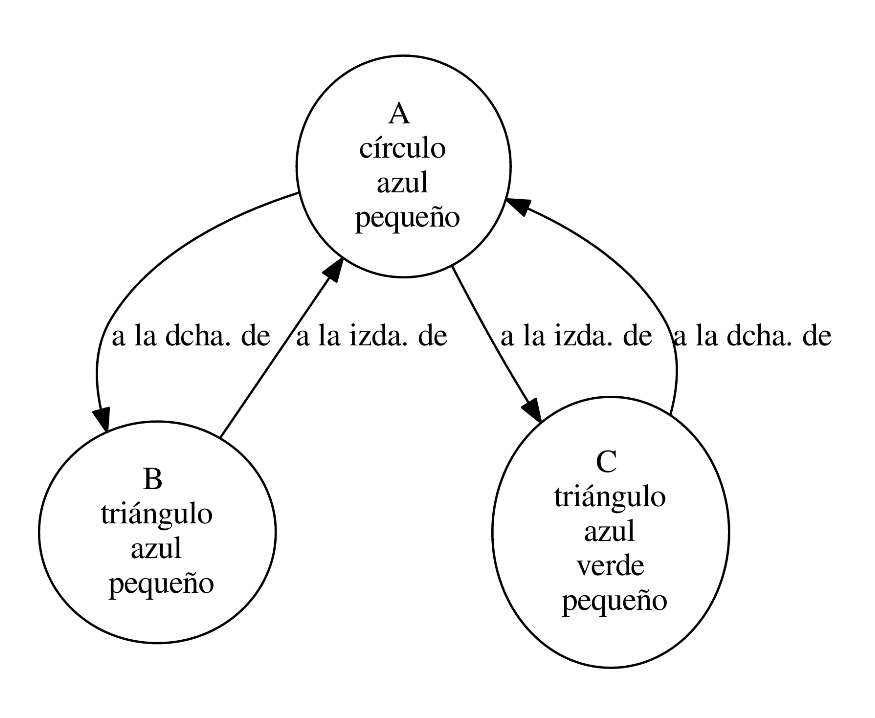
\includegraphics[width=0.5\textwidth]{img/riEjemploAlgoritmoDifusoCorte05.png}
			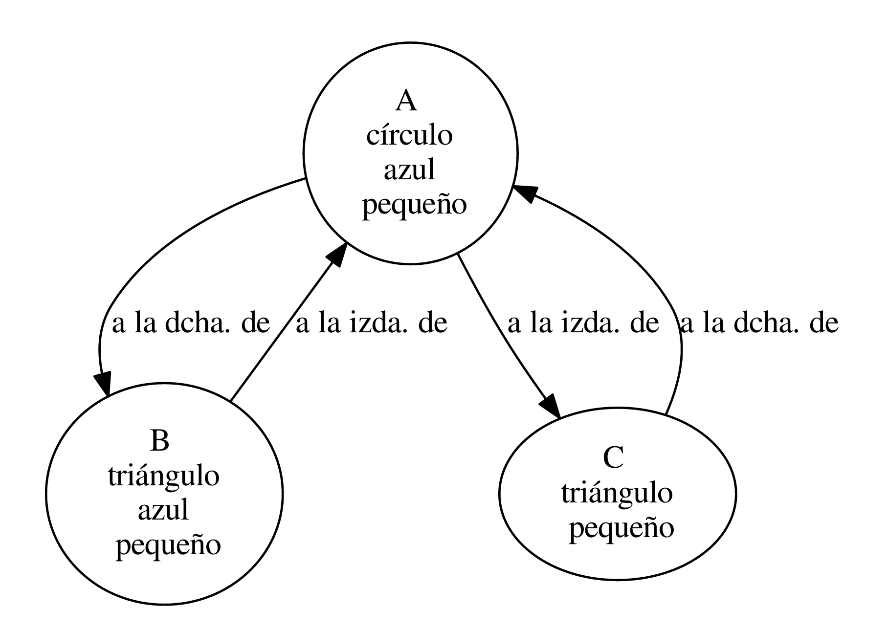
\includegraphics[width=0.5\textwidth]{img/riEjemploAlgoritmoDifusoCorte1.png}
		\end{figure}		
	\end{frame}
	
	\begin{frame}
		\begin{figure}
			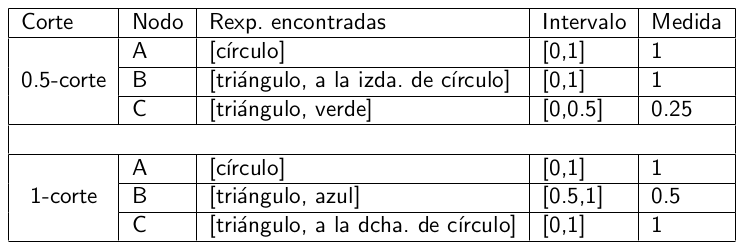
\includegraphics[width=1\textwidth]{img/tabla.png}			
		\end{figure}
	\end{frame}
	
	\subsection{Información difusa}
	
	\begin{frame}
		\begin{figure}
			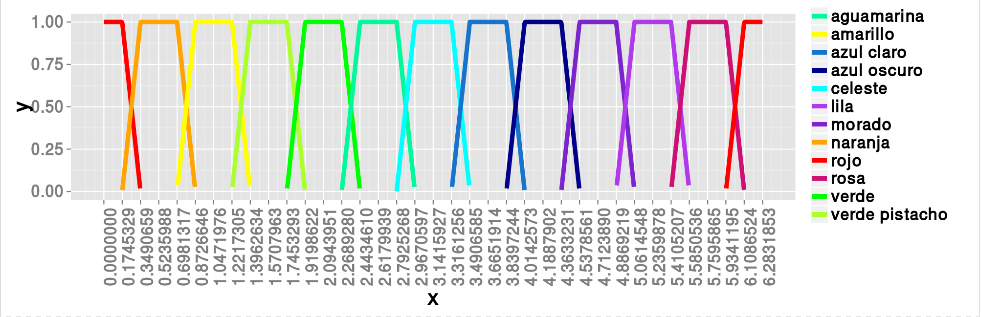
\includegraphics[width=1\textwidth]{img/partitionColor.png}			
		\end{figure}
	\end{frame}
	
	\begin{frame}
		\begin{figure}
			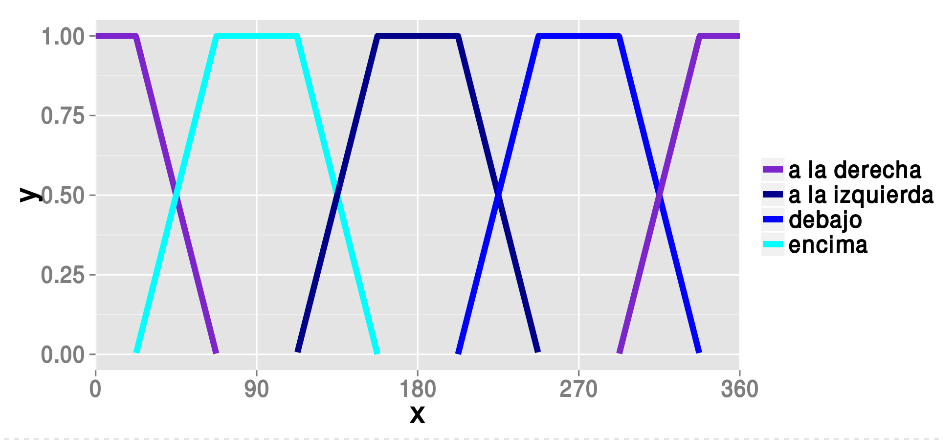
\includegraphics[width=1\textwidth]{img/partitionRelPos.png}			
		\end{figure}
	\end{frame}
	
	\begin{frame}
		\begin{figure}
			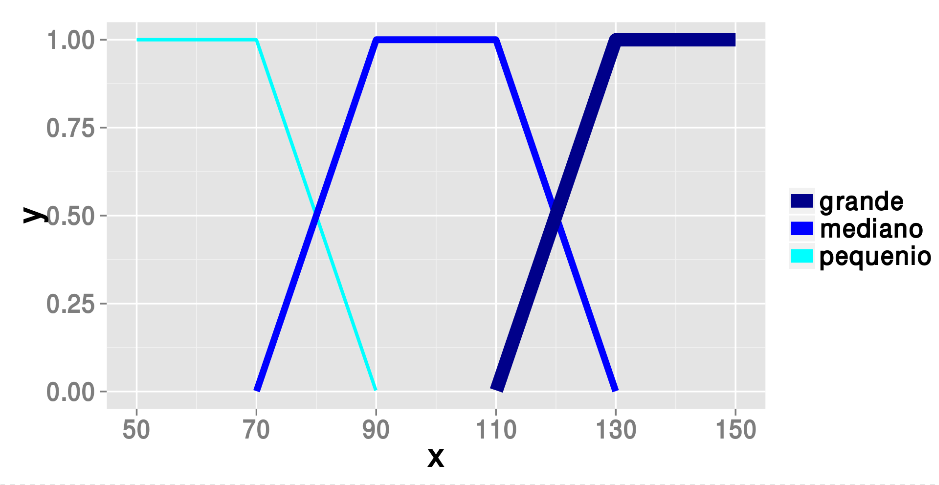
\includegraphics[width=1\textwidth]{img/partitionTam.png}			
		\end{figure}
	\end{frame}
	
	\subsection{Demo}
	
	\begin{frame}
		\begin{center}
			\href{https://www.youtube.com/watch?v=sfQNCcHsYu8}{Vídeo demo.}
		\end{center}
	\end{frame}
	
	\section*{}
	
	\begin{frame}[plain]
		\frametitle{Bibliografía}
		\nocite{*}
		\bibliographystyle{unsrt}
		\bibliography{biblioResumen}
	\end{frame}
	
	\begin{frame}[plain]
		\begin{center}
			Gracias. ¿Preguntas?
		\end{center}
	\end{frame}
		
		
	
	
	
	
\end{document}